% !Mode:: "TeX:UTF-8"
\documentclass[12pt,a4paper]{article}

%%%%%%%%------------------------------------------------------------------------
%%%% 日常所用宏包

%% 控制页边距
% 如果是beamer文档类, 则不用geometry
\makeatletter
\@ifclassloaded{beamer}{}{\usepackage[top=2.5cm, bottom=2.5cm, left=2.5cm, right=2.5cm]{geometry}}
\makeatother

%% 控制项目列表
\usepackage{enumerate}

%% 多栏显示
\usepackage{multicol}

%% 算法环境
\usepackage{algorithm}  
\usepackage{algorithmic} 
\usepackage{float} 

%% 网址引用
\usepackage{url}

%% 控制矩阵行距
\renewcommand\arraystretch{1.4}

%% hyperref宏包,生成可定位点击的超链接,并且会生成pdf书签
\makeatletter
\@ifclassloaded{beamer}{
\usepackage{hyperref}
\usepackage{ragged2e} % 对齐
}{
\usepackage[%
    pdfstartview=FitH,%
    CJKbookmarks=true,%
    bookmarks=true,%
    bookmarksnumbered=true,%
    bookmarksopen=true,%
    colorlinks=true,%
    citecolor=blue,%
    linkcolor=blue,%
    anchorcolor=green,%
    urlcolor=blue%
]{hyperref}
}
\makeatother



\makeatletter % 如果是 beamer 不需要下面两个包
\@ifclassloaded{beamer}{
\mode<presentation>
{
} 
}{
%% 控制标题
\usepackage{titlesec}
%% 控制目录
\usepackage{titletoc}
}
\makeatother

%% 控制表格样式
\usepackage{booktabs}

%% 控制字体大小
\usepackage{type1cm}

%% 首行缩进,用\noindent取消某段缩进
\usepackage{indentfirst}

%% 支持彩色文本、底色、文本框等
\usepackage{color,xcolor}

%% AMS LaTeX宏包: http://zzg34b.w3.c361.com/package/maths.htm#amssymb
\usepackage{amsmath,amssymb}
%% 多个图形并排
\usepackage{subfig}
%%%% 基本插图方法
%% 图形宏包
\usepackage{graphicx}
\newcommand{\red}[1]{\textcolor{red}{#1}}
\newcommand{\blue}[1]{\structure{#1}}
\newcommand{\brown}[1]{\textcolor{brown}{#1}}
\newcommand{\green}[1]{\textcolor{green}{#1}}


%%%% 基本插图方法结束

%%%% pgf/tikz绘图宏包设置
\usepackage{pgf,tikz}
\usetikzlibrary{shapes,automata,snakes,backgrounds,arrows}
\usetikzlibrary{mindmap}
%% 可以直接在latex文档中使用graphviz/dot语言,
%% 也可以用dot2tex工具将dot文件转换成tex文件再include进来
%% \usepackage[shell,pgf,outputdir={docgraphs/}]{dot2texi}
%%%% pgf/tikz设置结束


\makeatletter % 如果是 beamer 不需要下面两个包
\@ifclassloaded{beamer}{

}{
%%%% fancyhdr设置页眉页脚
%% 页眉页脚宏包
\usepackage{fancyhdr}
%% 页眉页脚风格
\pagestyle{plain}
}

%% 有时会出现\headheight too small的warning
\setlength{\headheight}{15pt}

%% 清空当前页眉页脚的默认设置
%\fancyhf{}
%%%% fancyhdr设置结束


\makeatletter % 对 beamer 要重新设置
\@ifclassloaded{beamer}{

}{
%%%% 设置listings宏包用来粘贴源代码
%% 方便粘贴源代码,部分代码高亮功能
\usepackage{listings}

%% 设置listings宏包的一些全局样式
%% 参考http://hi.baidu.com/shawpinlee/blog/item/9ec431cbae28e41cbe09e6e4.html
\lstset{
showstringspaces=false,              %% 设定是否显示代码之间的空格符号
numbers=left,                        %% 在左边显示行号
numberstyle=\tiny,                   %% 设定行号字体的大小
basicstyle=\footnotesize,                    %% 设定字体大小\tiny, \small, \Large等等
keywordstyle=\color{blue!70}, commentstyle=\color{red!50!green!50!blue!50},
                                     %% 关键字高亮
frame=shadowbox,                     %% 给代码加框
rulesepcolor=\color{red!20!green!20!blue!20},
escapechar=`,                        %% 中文逃逸字符,用于中英混排
xleftmargin=2em,xrightmargin=2em, aboveskip=1em,
breaklines,                          %% 这条命令可以让LaTeX自动将长的代码行换行排版
extendedchars=false                  %% 这一条命令可以解决代码跨页时,章节标题,页眉等汉字不显示的问题
}}
\makeatother
%%%% listings宏包设置结束


%%%% 附录设置
\makeatletter % 对 beamer 要重新设置
\@ifclassloaded{beamer}{

}{
\usepackage[title,titletoc,header]{appendix}
}
\makeatother
%%%% 附录设置结束


%%%% 日常宏包设置结束
%%%%%%%%------------------------------------------------------------------------


%%%%%%%%------------------------------------------------------------------------
%%%% 英文字体设置结束
%% 这里可以加入自己的英文字体设置
%%%%%%%%------------------------------------------------------------------------

%%%%%%%%------------------------------------------------------------------------
%%%% 设置常用字体字号,与MS Word相对应

%% 一号, 1.4倍行距
\newcommand{\yihao}{\fontsize{26pt}{36pt}\selectfont}
%% 二号, 1.25倍行距
\newcommand{\erhao}{\fontsize{22pt}{28pt}\selectfont}
%% 小二, 单倍行距
\newcommand{\xiaoer}{\fontsize{18pt}{18pt}\selectfont}
%% 三号, 1.5倍行距
\newcommand{\sanhao}{\fontsize{16pt}{24pt}\selectfont}
%% 小三, 1.5倍行距
\newcommand{\xiaosan}{\fontsize{15pt}{22pt}\selectfont}
%% 四号, 1.5倍行距
\newcommand{\sihao}{\fontsize{14pt}{21pt}\selectfont}
%% 半四, 1.5倍行距
\newcommand{\bansi}{\fontsize{13pt}{19.5pt}\selectfont}
%% 小四, 1.5倍行距
\newcommand{\xiaosi}{\fontsize{12pt}{18pt}\selectfont}
%% 大五, 单倍行距
\newcommand{\dawu}{\fontsize{11pt}{11pt}\selectfont}
%% 五号, 单倍行距
\newcommand{\wuhao}{\fontsize{10.5pt}{10.5pt}\selectfont}
%%%%%%%%------------------------------------------------------------------------


%% 设定段间距
\setlength{\parskip}{0.5\baselineskip}

%% 设定行距
\linespread{1}


%% 设定正文字体大小
% \renewcommand{\normalsize}{\sihao}

%制作水印
\RequirePackage{draftcopy}
\draftcopyName{XTUMESH}{100}
\draftcopySetGrey{0.90}
\draftcopyPageTransform{40 rotate}
\draftcopyPageX{350}
\draftcopyPageY{80}

%%%% 个性设置结束
%%%%%%%%------------------------------------------------------------------------


%%%%%%%%------------------------------------------------------------------------
%%%% bibtex设置

%% 设定参考文献显示风格
% 下面是几种常见的样式
% * plain: 按字母的顺序排列,比较次序为作者、年度和标题
% * unsrt: 样式同plain,只是按照引用的先后排序
% * alpha: 用作者名首字母+年份后两位作标号,以字母顺序排序
% * abbrv: 类似plain,将月份全拼改为缩写,更显紧凑
% * apalike: 美国心理学学会期刊样式, 引用样式 [Tailper and Zang, 2006]

\makeatletter
\@ifclassloaded{beamer}{
\bibliographystyle{apalike}
}{
\bibliographystyle{unsrt}
}
\makeatother


%%%% bibtex设置结束
%%%%%%%%------------------------------------------------------------------------

%%%%%%%%------------------------------------------------------------------------
%%%% xeCJK相关宏包

\usepackage{xltxtra,fontspec,xunicode}
\usepackage[slantfont, boldfont]{xeCJK} 

%% 针对中文进行断行
\XeTeXlinebreaklocale "zh"             

%% 给予TeX断行一定自由度
\XeTeXlinebreakskip = 0pt plus 1pt minus 0.1pt

%%%% xeCJK设置结束                                       
%%%%%%%%------------------------------------------------------------------------

%%%%%%%%------------------------------------------------------------------------
%%%% xeCJK字体设置

%% 设置中文标点样式,支持quanjiao、banjiao、kaiming等多种方式
\punctstyle{kaiming}                                        
                                                     
%% 设置缺省中文字体
\setCJKmainfont[BoldFont={Adobe Heiti Std}, ItalicFont={Adobe Kaiti Std}]{Adobe Song Std}   
%% 设置中文无衬线字体
\setCJKsansfont[BoldFont={Adobe Heiti Std}]{Adobe Kaiti Std}  
%% 设置等宽字体
\setCJKmonofont{Adobe Heiti Std}                            

%% 英文衬线字体
\setmainfont{DejaVu Serif}                                  
%% 英文等宽字体
\setmonofont{DejaVu Sans Mono}                              
%% 英文无衬线字体
\setsansfont{DejaVu Sans}                                   

%% 定义新字体
\setCJKfamilyfont{song}{Adobe Song Std}                     
\setCJKfamilyfont{kai}{Adobe Kaiti Std}
\setCJKfamilyfont{hei}{Adobe Heiti Std}
\setCJKfamilyfont{fangsong}{Adobe Fangsong Std}
\setCJKfamilyfont{lisu}{LiSu}
\setCJKfamilyfont{youyuan}{YouYuan}

%% 自定义宋体
\newcommand{\song}{\CJKfamily{song}}                       
%% 自定义楷体
\newcommand{\kai}{\CJKfamily{kai}}                         
%% 自定义黑体
\newcommand{\hei}{\CJKfamily{hei}}                         
%% 自定义仿宋体
\newcommand{\fangsong}{\CJKfamily{fangsong}}               
%% 自定义隶书
\newcommand{\lisu}{\CJKfamily{lisu}}                       
%% 自定义幼圆
\newcommand{\youyuan}{\CJKfamily{youyuan}}                 

%%%% xeCJK字体设置结束
%%%%%%%%------------------------------------------------------------------------

%%%%%%%%------------------------------------------------------------------------
%%%% 一些关于中文文档的重定义
\newcommand{\chntoday}{\number\year\,年\,\number\month\,月\,\number\day\,日}
%% 数学公式定理的重定义

%% 中文破折号,据说来自清华模板
\newcommand{\pozhehao}{\kern0.3ex\rule[0.8ex]{2em}{0.1ex}\kern0.3ex}

\newtheorem{example}{例}                                   
\newtheorem{theorem}{定理}[section]                         
\newtheorem{definition}{定义}
\newtheorem{axiom}{公理}
\newtheorem{property}{性质}
\newtheorem{proposition}{命题}
\newtheorem{lemma}{引理}
\newtheorem{corollary}{推论}
\newtheorem{remark}{注解}
\newtheorem{condition}{条件}
\newtheorem{conclusion}{结论}
\newtheorem{assumption}{假设}

\makeatletter %
\@ifclassloaded{beamer}{

}{
%% 章节等名称重定义
\renewcommand{\contentsname}{目录}     
\renewcommand{\indexname}{索引}
\renewcommand{\listfigurename}{插图目录}
\renewcommand{\listtablename}{表格目录}
\renewcommand{\appendixname}{附录}
\renewcommand{\appendixpagename}{附录}
\renewcommand{\appendixtocname}{附录}
%% 设置chapter、section与subsection的格式
\titleformat{\chapter}{\centering\huge}{第\thechapter{}章}{1em}{\textbf}
\titleformat{\section}{\centering\sihao}{\thesection}{1em}{\textbf}
\titleformat{\subsection}{\xiaosi}{\thesubsection}{1em}{\textbf}
\titleformat{\subsubsection}{\xiaosi}{\thesubsubsection}{1em}{\textbf}

\@ifclassloaded{book}{

}{
\renewcommand{\abstractname}{摘要}
}
}
\makeatother

\renewcommand{\figurename}{图}
\renewcommand{\tablename}{表}

\makeatletter
\@ifclassloaded{book}{
\renewcommand{\bibname}{参考文献}
}{
\renewcommand{\refname}{参考文献} 
}
\makeatother

\floatname{algorithm}{算法}
\renewcommand{\algorithmicrequire}{\textbf{输入:}}
\renewcommand{\algorithmicensure}{\textbf{输出:}}

%%%% 中文重定义结束
%%%%%%%%------------------------------------------------------------------------


\title{线弹性动力学变分原理}
%\author{}
\date{\chntoday}

\begin{document}
\maketitle

为了讨论方便,用小写字母下标 $i,~j$ 表示与各空间坐标方向对应的物理量,如用 $x_i$ 表示 $(x, y, z)$,用 $u_i$ 表示 $(u, v, w)$.

求导记号的缩写约定:
$$(~)_{,j}=\frac{\partial}{\partial x_j}(~),~u_{i,j}=\frac{\partial u_i}{\partial x_j}$$

$$(~)_{,ij}=\frac{\partial^2 (~)}{\partial x_i\,\partial x_j},~u_{k,ij}=\frac{\partial^2 u_k}{\partial x_i\,\partial x_j}$$

因此线弹性动力学的控制方程可以重写为:

运动方程
\begin{equation}
\sigma_{ij,j}+\bar{f}_i=\rho\ddot{u}_i ~~in~V
\end{equation}

应变-位移关系
\begin{equation}
\varepsilon_{ij}=\frac{1}{2}(u_{i,j}+u_{j,i})
\end{equation}

应力-应变关系
\begin{equation}
\sigma_{ij}=D_{ijkl}\varepsilon_{kl}
\end{equation}

边界条件
\begin{equation}
\sigma_{ij}n_j=\bar{T}_i ~~on~S_{\sigma}
\end{equation}
\begin{equation}
u_i=\bar{u}_i ~~on~S_u 
\end{equation}

初始条件
\begin{equation}
u_i|_{t=0}=\bar{u}^0_i
\end{equation}
\begin{equation}
\dot{u}_i|_{t=0}=\dot{\bar{u}}^0_i
\end{equation}

其中 $\sigma_{ij},\varepsilon_{ij}$ 和 $u_i$ 分别为应力张量、应变张量和位移矢量,$\bar{f}_i,\bar{T}_i$ 和 $\bar{u}_i$分别是域 $V$ 中的体力、边界 $S_{\sigma}$ 上的给定面力和边界 $S_u$ 上的给定位移,它们都是时间 $t$ 和空间坐标 $x_i (i = 1, 2, 3)$ 的函数。$\bar{u}^0_i$ 和 $\dot{\bar{u}}^0_i$ 分别为初位移矢量和初速度矢量。

\section{加权余量法}
对于复杂的实际问题,只能采用数值方法来求其近似解。近似解通常不能精确满足运动方程 $(1)$ 和边界条件 $(4)$,即
\begin{equation}
R_i=\sigma_{ij,j}+\bar{f}_i-\rho\ddot{u}_i\ne 0 ~~in~V
\end{equation}
\begin{equation}
\bar{R}_i=\sigma_{ij}n_j-\bar{T}_i\ne 0 ~~on~S_{\sigma}
\end{equation}
$R_i$ 和 $\bar{R}_i$ 分别为运动方程 $(1)$ 和边界条件 $(4)$ 的余量。

加权余量法是求解微分方程近似解的一种常用方法,它允许运动方程和边界条件在各点都存在余量,但要求这些余量在 $V$ 中和边界 $S_{\sigma}$ 上的加权积分为零,即要求满足余量方程:
\begin{equation}
\int_{V} R_iv_i ~ \mathrm{d}V=0,~~ i=1,2,3
\end{equation}
\begin{equation}
\int_{S_{\sigma}} \bar{R}_i\bar{v}_i ~ \mathrm{d}S=0,~~ i=1,2,3
\end{equation}
称 $v_i$ 和 $\bar{v}_i$ 分别为定义在 $V$ 内和边界 $S_{\sigma}$ 上的权函数。

若积分方程 $(10)$ 和 $(11)$ 对任意权函数 $v_i$ 和 $\bar{v}_i$ 都成立,则 $R_i\equiv 0 ~~in~V,~\bar{R}_i\equiv 0 ~~on~S_{\sigma}$,即微分方程 $(1)$ 在 $V$ 内任一点任一时刻都满足,边界条件 $(4)$ 在边界 $S_{\sigma}$上任一点任一时刻都满足,因此式 $(10)$ 和式 $(11)$ 是微分方程 $(1)$ 和边界条件 $(4)$的等效积分形式。

一般可将近似解取为一族已知函数的线性组合,即
\begin{equation}
u_i=\sum_{I=1}^N \Phi_I a_{iI}
\end{equation}
其中 $a_{iI}$ 为待定参数,也就是真正的求解目标,它们由式 $(10)$ 和式 $(11)$ 确定。$\Phi_I$ 为定义在整个求解域上的已知函数,称为试探函数(或基函数、形函数),它取自完全的函数序列 (即任一函数都可以用此函数序列展开),并且是线性独立的。当确定 $a_{iI}$ 以后,就可以得到原问题的近似解答。近似函数所取试探函数的项数 $N$ 越多,近似解的精度将越高;若 $N$ 区域无穷,近似解将收敛于精确解。

加权余量法实质上是通过选择合适的待定参数强迫余量在某种平均意义下为零。

任何相互独立的完备函数集都可以作为权函数,选取不同的权函数就得到不同的加权余量法。为了简单起见,在下面的讨论中,假设近似函数精确满足边界条件 (即 $\bar{R}_i = 0$),因此只考虑域内余量。权函数 $v_i$ 可以取为 $N$ 个函数的线性组合,即
\begin{equation}
v_i=\sum_{I=1}^N W_I b_{iI}
\end{equation}
$b_{iI}$ 为待定系数。将上式代入式 $(10)$ 中,考虑到待定系数 $b_{iI}$ 的任意性,得
\begin{equation}
\int_{V} R_iW_I ~ \mathrm{d}V=0,~~i=1,2,3;~~I=1,2,\cdots ,N
\end{equation}
此时,$W_I$ 也是权函数,下面将讨论几种常用的权函数。

\subsection{配点法}
权函数取为 $Dirac-\delta$函数:
\begin{equation}
W_I=\delta(x-x_I),~~I=1,2,\cdots ,N
\end{equation}
$$
\delta(x-x_I)
=\begin{cases}
0,~~x\ne x_I \\
\infty ,~~x=x_I
\end{cases}
$$
将上式代入式 $(14)$ 中,可得
\begin{equation}
R_i(x_I)=0,~~i=1,2,3;~~I=1,2,\cdots ,N
\end{equation}
这种方法是使余量在 $V$ 内指定的 $N$ 个离散点上为零,这些点称为配点。上式共有 $3N$ 个方程,可以解出 $3N$ 个待定系数 $a_{iI}$.
配点法只在配点上保证余量为零,不需要作积分计算,所以是加权余量法中最简单的一种,只是其计算精度相对差一些。

\subsection{子域法}
子域法首先将求解域 $V$ 划分为 $N$ 个子域 $V_I$,划分的子域总数等于待定系数 $a_{iI}$ 的总数,在每个子域内令权函数等于 $1$,在子域之外取权函数为零,也即:
\begin{equation}
W_I=\begin{cases}
1,~~x\in V_I \\
0,~~x\ne V_I
\end{cases}
\end{equation}
子域法实质是使余量在这 $N$ 个子域 $V_I$ 上的积分为零,即 $\int_{V_I} R_i~ \mathrm{d}V_I=0,~~I=1,2,\cdots ,N$

\subsection{最小二乘法}
最小二乘法通过调整近似函数中的参数 $a_{iI}$,使余量的均方和为最小,由极值条件有:
\begin{equation}
\frac{\partial}{\partial a_{iI}}\int_{V} R^2_i ~ \mathrm{d}V=2\int_{V} R_i\frac{\partial R_i}{\partial a_{iI}} ~ \mathrm{d}V=0
\end{equation}
与式 $(14)$ 相比,可知最小二乘法的权函数为
\begin{equation}
W_I=\frac{\partial R_i}{\partial a_{iI}},~~I=1,2,\cdots ,N
\end{equation}
最小二乘法的实质是使余量最小,这个方法一般计算精度高,但运算较为繁琐。

\subsection{伽辽金法}
伽辽金法利用近似解的试探函数序列 $\Phi _I$ 作为权函数,即
\begin{equation}
W_I=\Phi _I
\end{equation}
相应的余量方程为
\begin{equation}
\int_{V} R_i\Phi _I ~ \mathrm{d}V=0,~~i=1,2,3;~~I=1,2,\cdots ,N
\end{equation}

在许多情况下,伽辽金法得到的求解方程的系数矩阵是对称的,因而在用加权余量法建立有限元格式时主要采用伽辽金法。另外当存在相应的泛函时,伽辽金法与变分法往往给出同样的结果。

\begin{figure}[H]
\centering
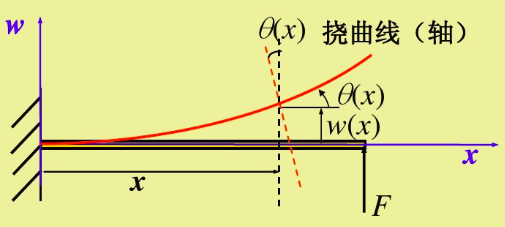
\includegraphics[scale=0.5]{./figures/2.png}
\caption{}
\end{figure}

弯曲使梁的任意 x 截面产生弯曲位移:

$(1)$ 扰度 $\omega(x)$ — 截面形心的铅垂位移,即弯曲变形时横截面形心沿与轴线垂直方向的线位移称为挠度;向上为正。

$(2)$ 转角 $\theta(x)$ — 截面绕中性轴转过的角度,以逆时针方向为正。

当小变形时,有 $\theta\thickapprox tan\theta =\frac{d\omega}{dx}$

例 $1$ 用各种加权余量法求解下图中的弹性基础梁的挠度。
\begin{figure}[H]
\centering

\includegraphics[scale=0.6]{./figures/1.png}
\caption{}
\end{figure}

解: 图示弹性基础梁的基本微分方程和边界条件为
\begin{equation}
\begin{cases}
\frac{d^4w}{dx^4}+\alpha w+1=0,~~-1\leqslant x\leqslant 1 \\
w(-1)=0 \\
w(1)=0
\end{cases}
\end{equation}

上 式 采 用 了 无 量 纲 形 式,其 中 无 量 纲 参 数 $x$ 、$w$ 和 $M$ 应 分 别 乘 上 系 数 $L/2$ 、
$pL^4/(16EI)$ 和 $pL^2/4$ 才是实际的坐标、挠度和弯矩。参数 $\alpha = kL^4/(16EI)$,$k$ 为基础刚
度系数,$EI$ 为梁抗弯刚度。

作为一阶近似,把试探函数 $\phi_1$ 取为当 $\alpha = k = 0$ 时的精确解,即 $\phi_1(x)= −\frac{1}{24}(5-x^2)(1−x^2)$.近似解为
$$
w_1(x)=\phi_1a_1= −\frac{a_1}{24}(5-x^2)(1−x^2)
$$
上式满足边界条件,因此只有域内存在余量。把上式代入式 $(22)$ 中,得到微分方程的残差为
$$
R_1(x,a_1)=-a_1-\alpha\frac{a_1}{24}(5-x^2)(1−x^2)+1
$$

$1$. 配点法 ~~ 要求在 $x=0$ 处余量为零,即取 $x=0$ 作为配点,因此有
$$
R_1(0,a_1)=-a_1-\frac{5\alpha}{24}a_1+1=0
$$
得
$$
a_1=(1+\frac{5\alpha}{24})^{-1}
$$

$2$. 子域法 ~~ 要求余量在区域中的积分为零,即取整个问题域作为子域,因此有
$$
\int_{-1}^{1} R_1 ~\mathrm{d}x=-a_1-\frac{2\alpha}{15}a_1+1=0
$$
得
$$
a_1=(1+\frac{2\alpha}{15})^{-1}
$$

$3$. 最小二乘法
$$
\frac{\partial R_1}{\partial a_1}=-1-\frac{\alpha}{24}(5-x^2)(1−x^2)
$$
由 $\int_{-1}^{1} R_1\frac{\partial R_1}{\partial a_1}dx=0$ 得
$$
a_1=(1+\frac{2\alpha}{15})(1+\frac{4\alpha}{15}+\frac{62\alpha ^2}{2835})^{-1}
$$

$4$. 伽辽金法  权函数取为 $\phi_1=−\frac{1}{24}(5-x^2)(1−x^2)$,由余量方程 $\int_{-1}^{1} R_1\phi_1dx=0$ 得
$$
a_1=(1+\frac{31\alpha}{189})^{-1}
$$

为了得到更精确的结果,需要进一步改进试探函数,增加新的函数项。

\section{达朗贝尔—拉格朗日原理}
函数 $y(x)$ 的变分定义为 $\delta y=y_1(x)-y(x)$,其中 $y_1(x)$ 是“靠近” $y(x)$ 的一个函数,即 
$\delta y$ 是同一自变量 $x$ 处相邻函数的函数值之差,也就是说变分是函数的增量。

\begin{figure}[H]
\centering
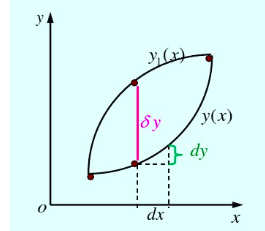
\includegraphics[scale=0.6]{./figures/3.png}
\caption{}
\end{figure}

变分具有以下的性质:
$$
\delta (u+w)=\delta u+\delta w
$$
$$
\delta (uw)=w\delta u+u\delta w
$$
$$
\delta (\frac{u}{w})=\frac{w\delta u-u\delta w}{w^2}
$$
$$
\delta\frac{\partial u}{\partial x}=\frac{\partial}{\partial x}\delta u
$$
$$
\delta (dy)=d(\delta y)
$$
$$
\delta\int udS=\int\delta udS
$$



变分与微分的区别:$y=y(x)$,$dy$ 与 $\delta y$ 的区别

变分 $dy$ 是函数 $y$ 本身形状发生变化而引起的微小变化;而微分 $dy$ 是自变量 $x$ 发生变化而引起的函数的微小变化。

虚位移:

虚位移是符合约束条件的无穷小位移。由于任何物理运动都需要经过时间的演进才会有实际的位移,所以称保持时间不变的位移为虚位移。因此虚位移只是空间位移;时间是固定的。

虚位移要求是微小的位移,即要求在产生虚位移过程中不改变原受力平衡体的力的作用方向与大小,亦即受力平衡体平衡状态不会因产生虚位移而改变。

虚位移用 $\delta u_i$ 表示,以区别于实位移 $du_i$.

定常约束:

又称稳定约束,不随时间变化的一种约束。

非定常系统:

假若一个系统的任何约束是非定常约束,则称此系统为非定常系统。非定常约束的方程式显性地含时间。

虚功:

真实力在虚位移上所作的功称为虚功,表达式为
$$
\delta W_F=\textbf{F}\cdot\delta\textbf{r}
$$

现在假设位移分量发生了位移边界条件所容许的微小改变(虚位移),记为 $\delta u_i$.\\


利用加权余量法,将权函数取为真实位移的变分 $\delta u_i$,则得运动方程 $(1)$ 和力边界条
件 $(4)$ 的等效积分形式
\begin{equation}
\int_{V}\delta u_i(\sigma_{ij,j}+\bar{f}_i-\rho\ddot{u}_i)dV=0
\end{equation}
\begin{equation}
\int_{S_{\sigma}}\delta u_i(\sigma_{ij}n_j-\bar{T}_i)dS=0
\end{equation}

式中的积分在 $t$ 瞬时分别遍及整个区域 $V$ 和边界 $S_{\sigma}$.利用分部积分,并考虑到 $\delta u_i|S_u=0$(在 $S_u$ 处位移 $u_i$ 已知,其变分为零),$S=S_{\sigma}\cup S_u$,~$\delta u_{i,j}\sigma_{ij}=\delta\varepsilon_{ij}\sigma_{ij}$,有
$$
\int_{V} \delta u_i\sigma_{ij,j}dV =\int_{V} [(\delta u_i\sigma_{ij})_{,j}-\delta u_{i,j}\sigma_{ij}]dV =\int_{S} \delta u_i\sigma_{ij}n_jdS-\int_{V}\delta\varepsilon_{ij}\sigma_{ij}dV
$$
\begin{equation}
\int_{V} \delta u_i\sigma_{ij,j}dV=\int_{S_{\sigma}} \delta u_i\sigma_{ij}n_jdS-\int_{V}\delta\varepsilon_{ij}\sigma_{ij}dV
\end{equation}

将式 $(25)$ 代入式 $(23)$,并引入式 $(24)$,最终得到
\begin{equation}
-\int_{V}\delta u_i\rho\ddot{u}_idV-\int_{V}\delta\varepsilon_{ij}\sigma_{ij}dV+\int_{V} \bar{f}_i\delta u_idV+\int_{S_{\sigma}}\bar{T}_i\delta u_idS=0
\end{equation}
式中第一项为惯性力系的虚功,第二项为内力系的虚功,最后两项为外力系的虚功。上式即为线弹性动力学的达朗贝尔-拉格朗日原理,它表明力系 (外力、内力、惯性力) 在虚位移 $\delta u_i$ 和虚应变 $\delta\varepsilon_{ij}$ 上所做的虚功和为零。虚位移 $\delta u_i$ 和虚应变 $\delta\varepsilon_{ij}$ 应满足如下条件
\begin{equation}
\delta\varepsilon_{ij}=\frac{1}{2}(\delta u_{i,j}+\delta u_{j,i})
\end{equation}
\begin{equation}
\delta u_i|_{S_u}=0
\end{equation}

在导出达朗贝尔-拉格朗日原理时,未涉及物理方程(应力-应变关系),所以达朗贝尔-拉格朗日原理不仅可以用于线弹性问题,而且可以用于非线性弹性及弹塑性等非线性问题。

\section{哈密顿原理}

将式 $(26)$ 在时间间隔 $t_1$ 到 $t_2$ 之间对时间 $t$ 积分,有
\begin{equation}
-\int_{t_1}^{t_2} \int_{V}\delta u_i\rho\ddot{u}_idVdt-\int_{t_1}^{t_2} \int_{V}\delta\varepsilon_{ij}\sigma_{ij}dVdt+\int_{t_1}^{t_2} \int_{V}\bar{f}_i\delta u_idVdt+\int_{t_1}^{t_2} \int_{S_{\sigma}}\bar{T}_i\delta u_idSdt=0
\end{equation}

对上式第一项进行分部积分,并给定 $u_i$ 在 $t=t_1$ 和 $t=t_2$ 时刻的值 (即令 $\delta u_i|_{t=t_1}=0,~\delta u_i|_{t=t_2}=0$),得
$$
-\int_{t_1}^{t_2} \int_{V}\delta u_i\rho\ddot{u}_idVdt=-\int_{V} \int_{t_1}^{t_2}\delta u_i\rho\ddot{u}_idtdV=-\int_{V} \int_{t_1}^{t_2}\rho\left[\frac{d}{dt}(\delta u_i\dot{u}_i)-\delta\dot{u}_i\dot{u}_i\right]dtdV
$$
\begin{equation}
-\int_{t_1}^{t_2} \int_{V}\delta u_i\rho\ddot{u}_idVdt=-\int_{V}\rho(\delta u_i\dot{u}_i)|^{t_2}_{t_1}dV+\int_{V} \int_{t_1}^{t_2}\rho\delta\dot{u}_i\dot{u}_idtdV=\int_{t_1}^{t_2} \delta Tdt
\end{equation}
其中 $T$ 为弹性体的动能:
\begin{equation}
T=\frac{1}{2}\int_{V}\rho\dot{u}_i\dot{u}_idV
\end{equation}

$$
\delta T=\frac{1}{2}\int_{V}\rho(\delta\dot{u}_i)\dot{u}_idV+\frac{1}{2}\int_{V}\rho\dot{u}_i(\delta\dot{u}_i)dV=\int_{V}\rho(\delta\dot{u}_i)\dot{u}_idV
$$

将式 $(30)$ 代入式 $(29)$ 得到普遍意义下的哈密顿原理:
\begin{equation}
\int_{t_1}^{t_2} (\delta T+\delta W)dt=0
\end{equation}
式中
\begin{equation}
\delta W=-\int_{V}\delta\varepsilon_{ij}\sigma_{ij}dVdt+\int_{V}\bar{f}_i\delta u_idVdt+\int_{S_{\sigma}}\bar{T}_i\delta u_idSdt
\end{equation}
为系统内力及外力虚功。式 $(32)$ 表明,对于真实运动,系统的动能变分 $\delta T$ 和内力及外力虚功 $\delta W$ 之和在任一时间间隔内对时间的积分等于零。

粘滞力是由于流体的各流层的流速不同,相邻流层间有相对运动,便在接触面上产生一种相互作用的剪切力,这个力叫做流体的内摩擦力,也称为粘滞力。

考虑粘滞力后,哈密顿原理可以改写为
\begin{equation}
\int_{t_1}^{t_2} (\delta T+\delta W+\delta W_{\nu})dt=0
\end{equation}
其中 $=\delta W_{\nu}=-\int_{V}\nu\dot{u}_i\delta u_idV$ 为粘滞力 $-\nu\dot{u}_i$ 的虚功。

若系统的外力有势,外力虚功等于外力势能变分的负值,同时考虑到应力应变关系式 $(3)$,则式 $(33)$ 可改写为
\begin{equation}
\delta W=-\delta \Pi _P
\end{equation}

其中
\begin{equation}
\Pi _P=\int_{V}\frac{1}{2}D_{ijkl}\varepsilon_{ij}\varepsilon_{kl}dV-\int_{V}\bar{f}_iu_idV-\int_{S_{\sigma}}\bar{T}_iu_idS
\end{equation}
是系统的总势能,等于弹性体变形能和外力势能之和。

弹性变形能(应变能)是指在变形过程中,外力所作的功转变为储存于固体内的能量,固体在外力作用下,因变形而储存能量称为变形能或应变能。变形能有弹性变形能与塑性变形能。

将式 $(35)$ 代入式 $(32)$ 中得
\begin{equation}
\int_{t_1}^{t_2}\delta(T-\Pi _P)dt=0
\end{equation}\\


非完整系统:

一个系统有任何约束是非完整约束,则称此系统为非完整系统。

完整约束:

如果约束方程中不包含坐标对时间的导数,或者约束方程中微分项可以积分为有限形式,这类约束称为完整约束。\\


对于完整系统,上式中积分运算和变分运算可以交换顺序,故有
\begin{equation}
\delta S=0,~~S=\int_{t_1}^{t_2}(T-\Pi _P)dt
\end{equation}

式 $(38)$ 表明,完整有势系统在任意时间间隔内满足几何关系 $(2)$ 和给定位移边界条
件 $(5)$ 的所有可能运动中,真实运动使哈密顿作用量 $S$ 取驻值(一阶变分为零)。

上面从运动方程和力边界条件出发导出了哈密顿原理,下面由哈密顿原理出发导出运动方程和边界条件,从而证明哈密顿原理与运动方程及力边界条件是等价的。利用分部积分,式 $(37)$ 的第一项可进一步化为
$$
\delta\int_{t_1}^{t_2}Tdt=\int_{t_1}^{t_2}\int_{V}\rho\bar{u}_i\delta\bar{u}_idVdt=\int_{V}\rho\int_{t_1}^{t_2}\left[\frac{d}{dt}(\bar{u}_i\delta u_i)-\ddot{u}_i\delta u_i\right]dtdV
$$
\begin{equation}
\delta\int_{t_1}^{t_2}Tdt=\int_{V}\rho(\bar{u}_i\delta u_i)|^{t_2}_{t_1}dV-\int_{t_1}^{t_2}\int_{V}\rho\ddot{u}_i\delta u_idVdt
\end{equation}

考虑到 $\delta u_i|_{t=t_1}=\delta u_i|_{t=t_2}=0$,上式可简化为
\begin{equation}
\delta\int_{t_1}^{t_2}Tdt=-\int_{t_1}^{t_2}\int_{V}\rho\ddot{u}_i\delta u_idVdt
\end{equation}

对式 $(37)$ 的第二项进行分部积分为
$$
-\delta\int_{t_1}^{t_2}\Pi _Pdt=-\int_{t_1}^{t_2}\left(\int_{V}D_{ijkl}\varepsilon_{kl}\delta\varepsilon_{ij}dV-\int_{V}\bar{f}_i\delta u_idV-\int_{S_{\sigma}}\bar{T}_i\delta u_idS\right)dt
$$
$$
-\delta\int_{t_1}^{t_2}\Pi _Pdt=-\int_{t_1}^{t_2}\left(\int_{V}\sigma_{ij}\delta u_{i,j}dV-\int_{V}\bar{f}_i\delta u_idV-\int_{S_{\sigma}}\bar{T}_i\delta u_idS\right)dt
$$
\begin{equation}
-\delta\int_{t_1}^{t_2}\Pi _Pdt=-\int_{t_1}^{t_2}\left(-\int_{V}\sigma_{ij,j}\delta u_idV+\int_{S}\sigma_{ij}n_j\delta u_idS-\int_{V}\bar{f}_i\delta u_idV-\int_{S_{\sigma}}\bar{T}_i\delta u_idS\right)dt
\end{equation}

考虑到 $S=S_u\cup S_{\sigma}$,~$\delta u_i|_{S_u}=0$,上式可简化为
\begin{equation}
-\delta\int_{t_1}^{t_2}\Pi _Pdt=-\int_{t_1}^{t_2}\left(\int_{V}(-\sigma_{ij,j}-\bar{f}_i)\delta u_idV+\int_{S_{\sigma}}(\sigma_{ij}n_j-\bar{T}_i)\delta u_idS\right)dt
\end{equation}

把以上两式代入哈密顿原理式 $(37)$ 得
$$
\int_{t_1}^{t_2}\left(\int_{V}(-\rho\ddot{u}_i+\sigma_{ij,j}+\bar{f}_i)\delta u_idV-\int_{S_{\sigma}}(\sigma_{ij}n_j-\bar{T}_i)\delta u_idS\right)dt=0
$$

考虑到虚位移 $\delta u_i$ 的任意性,由上式可得
\begin{equation}
\sigma_{ij,j}+\bar{f}_i=\rho\ddot{u}_i
\end{equation}
\begin{equation}
\sigma_{ij,j}n_j=\bar{T}_i
\end{equation}

式 $(43)$ 和式 $(44)$ 称为哈密顿变分原理的欧拉方程和边界条件,它们就是运动方程及力边界条件。可见,对于线弹性动力学问题,原微分方程的等效积分弱形式 $(26)$ 可以进一步转化为泛函(哈密顿作用量 $S$)的驻值问题。这种求解微分方程的方法称为变分原理或变分法,它寻求使泛函取驻值的、满足一定已知边界条件 (在这里是指给定位移边界条件 $(5)$)的未知函数。

在推导哈密顿原理式 $(38)$ 时,用到了物理方程 $(3)$,因此哈密顿原理式 $(38)$ 只适用于线弹性问题,而达朗贝尔-拉格朗日原理不但适用于线弹性问题,也适用于非线弹性问题。

例 $2$ ~~ 用哈密顿原理推导左端固支、右端自由的等截面直杆(如下图所示)的欧拉方程。

\begin{figure}[H]
\centering
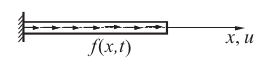
\includegraphics[scale=0.6]{./figures/6.png}
\caption{}
\end{figure}

解: 假定应力在截面上均匀分布,原来垂直于轴线的截面变形后仍保持和轴线垂直,因此可以简化为一维问题。杆内任一点的应变为
$$
\varepsilon_x=\frac{\partial u}{\partial x}
$$

系统的总势能为
\begin{equation}
\Pi _P=\int_{V}\frac{1}{2}E\varepsilon^2_xdV-\int_{0}^{l}f(x,t)udx=\int_{0}^{l}\frac{1}{2}EA(\frac{\partial u}{\partial x})^2dx-\int_{0}^{l}f(x,t)udx
\end{equation}
$$
\int_{V}\frac{1}{2}E\varepsilon^2_xdV=\frac{1}{2}\int_{0}^{l}\int_{S}E\varepsilon^2_xdSdx=\frac{1}{2}\int_{0}^{l}E\varepsilon^2_x\left(\int_{S}~dS\right)dx=\frac{1}{2}\int_{0}^{l}EA\varepsilon^2_xdx
$$
其中 $A$ 为截面面积。

系统的动能为
$$
T=\frac{1}{2}\int_{V}\rho\dot{u}^2dV=\frac{1}{2}\int_{0}^{l}\rho A\dot{u}^2dx
$$

$$
\frac{1}{2}\int_{V}\rho\dot{u}^2dV=\frac{1}{2}\int_{0}^{l}\int_{S}\rho\dot{u}^2dSdx=\frac{1}{2}\int_{0}^{l}\rho\dot{u}^2\left(\int_{S}~dS\right)dx
$$

对势能 $\Pi _P$ 取变分,利用分部积分,得
$$
\delta\Pi _P=\int_{0}^{l}EA\frac{\partial u}{\partial x}\delta\frac{\partial u}{\partial x}-\int_{0}^{l}f(x,t)\delta udx=EA\frac{\partial u}{\partial x}\delta u |^l_0-\int_{0}^{l}EA\frac{\partial^2 u}{\partial x^2}\delta udx-\int_{0}^{l}f(x,t)\delta udx
$$
$$
\int_{0}^{l}EA\frac{\partial u}{\partial x}d\delta u=EA\frac{\partial u}{\partial x}\delta u|^l_0-\int_{0}^{l}\delta ud\left(EA\frac{\partial u}{\partial x}\right)=EA\frac{\partial u}{\partial x}\delta u|^l_0-\int_{0}^{l}EA\delta ud\frac{\partial u}{\partial x}
$$

动能 $T$ 变分后在时间间隔 $t_1$ 到 $t_2$ 之间对 $t$ 积分,利用分部积分并考虑到 $\delta u|_{t=t_1}=\delta u|_{t=t_2}=0$,得
$$
\int_{t_1}^{t_2}\delta Tdt=\int_{t_1}^{t_2}\int_{0}^{l}\rho A\dot{u}\delta\dot{u}dxdt=\int_{0}^{l}\left[\rho A\dot{u}\delta u|^{t_2}_{t_1}\right]dx-\int_{t_1}^{t_2}\int_{0}^{l}\rho A\ddot{u}\delta udxdt=-\int_{t_1}^{t_2}\int_{0}^{l}\rho A\ddot{u}\delta udxdt
$$
$$
\int_{t_1}^{t_2}\rho A\dot{u}d\delta u=\rho A\dot{u}\delta u|_{t_1}^{t_2}-\int_{t_1}^{t_2}A\rho\delta ud\dot{u}
$$

将以上两式代入哈密顿原理式 $(37)$ 得
$$
\int_{t_1}^{t_2}\int_{0}^{l}\left[-\rho A\ddot{u}+EA\frac{\partial^2 u}{\partial x^2}+f(x,t)\right]\delta udxdt-\int_{t_1}^{t_2}EA\frac{\partial u}{\partial x}\delta u|_{0}^{l}dt=0
$$

考虑到虚位移 $\delta u$ 的任意性,上式第一项括号内的表达式必须等于零。另外杆的右截面自由,即 $\delta u|_{x=l}\ne 0$,因此 $EA\frac{\partial u}{\partial x}|_{x=l}$ 必须等于零。杆的左截面固定,即 $u|_{x=0}=0$.故得
$$
EA\frac{\partial^2 u}{\partial x^2}=\rho A\ddot{u}+f(x,t), ~~ 0<x<l
$$
$$
u|_{x=0}=0
$$
$$
EA\frac{\partial u}{\partial x}|_{x=l}=0
$$








































































%坎坎坷坷扩


%\cite{tam19912d}
%\bibliography{../ref}
\end{document}
